The DDG is initially a bipartite graph where all the decision variables $X$ are vertices in one set and all the 
constraints $C$ are vertices in the other set. If constraint $c$ applies to a variable $x$ then there is an arc from 
the vertex representing $x$ to the vertex representing $c$. \\    
We define as many variables to be one-way constraints as possible \boste{This is currently not true and think this 
will change (one could say it is possible to define all variables and that is the optimal solution)}, starting with 
integer variables such that the variables in the search space in local search only consists of binary variables 
\boste{Otherwise it is not possible to solve atm.}. \\
Let $X$ be a set of variables and $x \in X$. The subset of constraints $C(x) \subseteq C$ is the set 
of constraints that applies to $x$.\\ 
The following algorithms describe how one-way constraints a create to define a variable $x$. \\ 
\IncMargin{1em}
\begin{algorithm}[H]
\SetKwData{Oneway}{oneway}

\SetKwFunction{makeOneway}{makeOneway}
\SetKwFunction{Next}{next}\SetKwFunction{Constraints}{Constraints}\SetKwFunction{Remove}{remove}
\SetKwFunction{canBeMadeOneway}{canBeMadeOneway}
\algdata 
\Input{A set $X$ of variables \boste{Sorting order?}}
\Output{A model better suited for local search}
\BlankLine
%\emph{special treatment of the first line}\;
\Bool $change = $ \true\;
\While{$X \neq \emptyset$ \textbf{and} $change$}{
  $change = $\false \;
  \ForEach{$x \in X$}{
    \upshape select \Var $x$ \upshape from $X$\;
    \ForEach{\Con $c$ \upshape in $C(x)$}{
      \Bool $flag = $ \canBeMadeOneway{c,x}\;  
      \If{$flag$}{
	\makeOneway{c,x}\;
	Remove $x$ from $X$\;
	$change = \true$\;
	\bre\;
      }
    }
  }
}
\caption{Defining integer variables by one-way constraints}\label{algo_defintvar}
\end{algorithm}\DecMargin{1em}
\noindent
The algorithm tries to create invariants that define the set of variables $X$ by one-way constraints. It uses two other 
algorithms \canBeMadeOneway{c,x} and \makeOneway{c,x}. The first algorithm checks if the \cons $c$ can be used to define 
\var $x$ and the second algorithm transforms $c$ into a one-way constraint defining $x$. \\ 
The complexity of algorithm \ref{algo_defintvar} depends on the complexity of the two other algorithms but for 
simplicity let us assume they do not contribute for now. \\ 
Let $\alpha_{max}$ be the largest arity among all constraints in $C$ and $n$ be the number of decision variables in the 
input set. The size of $X$ has decrease by at least one each time we pass line 3 except for the first time. Hence line 3 
is passed at most $n$ times. Then the complexity of algorithm \ref{algo_defintvar} is $O(\alpha_{max} n^2)$. \\ \medskip
The coefficient of a variable $x_j$ in constraint $c_i$ is denoted $a_{ij}$. Let $\mathcal{F} = \{f_1,f_2,\dots ,f_k\}$ 
be the family of objective functions \boste{Think we should discuss this Tuesday} and the coefficient of variable $x_j$ 
in $f_k$ be $a_{kj}$. \boste{Maybe call it 
evaluation functions. Does not make sense since $a_{34}$ refers both to constraint and obj. func} \\  

\IncMargin{1em}
\begin{algorithm}[H]

\SetKwFunction{relation}{relation}\SetKwFunction{coeff}{coefficient}
\SetKwFunction{objcoeff}{objectiveCoefficients}
\algdata
\Input{\Con $c$ and \Var $x$}
\Output{Boolean}
\BlankLine
\If{c \upshape already defines a oneway constraint}{\Return{} \false\; \boste{This constraint could be removed in 
$O(\alpha(c))$}}
\If{\upshape Number of integer variables not defined $> 1$}{\Return{} \false\; \boste{Needed in order to create the 
right update queue}}
%\If{$|Y(c)| > 1$}{\Return{} \false}
\If{\relation{c} \upshape is (==) }{\Return{} \true}
%\int coeff = \coeff{c,v}\;
%\upshape in $\bigcup\limits_{o \in O} f_o(\vec{v})$}{	
\boste{The following is not at all correct, we should discuss this Tuesday} \\
\ForEach{a \upshape in $A(f(x))$ }{
  \If{$A(c,x) \cdot a > 0$}{
    \Return{} \false
  }
}
\Return{} \true\;
 \caption{canBeMadeOneway(\textsf{Constraint} c, \textsf{Variable} x)} \label{algo_checkoneway}
% \caption{Test if a constraint $c$ can define a variable $x$ } \label{algo_checkoneway}
\end{algorithm}
\DecMargin{1em}
\boste{Description not finished (done at all)}

%The variables that a constraint $c$ applies to is the scope $V(c)$. The constraints are of the type \class{Linear} and 
%a constraint $c$ have a right hand side $B(c)$. \\ 
\IncMargin{1em}
\begin{algorithm}[H]
\algdata
\Input{\Con $c$ and \Var $x$}
\Output{An Invariant}
\BlankLine
\int $coef = A_{c,x}$\;
$Q = A_c \backslash \{A_{c,x}\}$\;
$U = V(c) \backslash \{x\}$\;
\ForEach{$A_{c,x}$ \upshape in $Q$}{
  $Q_{c,x} = A(c,x) \cdot \frac{-1}{coef}$
}
\int $b = B(c)$ \;
\If{\relation{c} \upshape is (==) }{
  Invariant $c' = $ \Sum{$U$,$Q$,b}\;
  $G$ = $G \cup c'$\; 
  \boste{Maybe remove $c$ from $G$}
  %\Return{\Sum{$V(c)$,$A(c)$,b}}
}
\Else{
  Invariant $c' = $ \Sum{$U$,$Q$,b}\;
  Invariant $c'' = $ \Max{c',lb(x)}\;
  $G$ = $G \cup c'$\; 
  $G$ = $G \cup c''$\; 
  \boste{Maybe remove $c$ from $G$}
  %\Return{\Max{inv,b}}
}

 \caption{makeOneway(\textsf{Constraint} c, \textsf{Variable} x)} \label{algo_makeoneway}
 %\caption{Make one-way constraint from $c$ defining variable $x$ } \label{algo_makeoneway}
 \end{algorithm}\DecMargin{1em}
\boste{Description of algorithm here} \\
Consider the following three constraints as a small example. \boste{Should the example be introduced before the 
algorithms?}
\begin{center}
\begin{tabular}{rlr}
$ c_1: $&$2x_1 + y_2 -y_1 $&$= 2$ \\
$ c_2: $&$2x_1 - y_2 $&$= 2 $ \\ 
$ c_3: $&$x_1 +y_1 +y_2 $&$\leq 5 $
\end{tabular} 
\end{center}
At first $y_1$ cannot be defined by a \oneway but $y_2$ can be defined by $c_2$ and then $y_1$ can be defined by $c_1$. 
The order in which the \oneway are created matters. \boste{Not finished here, continue tomorrow morning} 
\begin{center}
    \begin{tikzpicture}[scale=1]
        \vertex[label=$x_1$](x1) at (-1,1) {};
        \vertex[label=$y_1$](y1) at (3,2) {};
        \vertex[label=$y_2$](y2) at (1,0) {};
        %\vertex[label=$c_3$](c3) at (5,1) {};
         %\vertex[label=$c_2$](c2) at (5,0) {};
    \tikzset{EdgeStyle/.style={->}}
        \Edge(x1)(y1)
        \Edge(y2)(y1)
        \Edge(x1)(y2)
        %\Edge(x1)(c3)
        %\Edge(y1)(c3)
        %\Edge(y2)(c3)
    \end{tikzpicture}
\end{center}

%algorithm \ref{algo_defintvar} first check if $y_1$ can be defined by a \oneway which it cannot since $c_1$ applies to 
%two integer variables. Then $y_2$ cannot be defined by $c_1$ but can be defined by $c_2$. Then $c_2$ is transformed 
%into a \oneway $c_2'$ that defines $y_2$ and it is added to the DDG $G$, $c_2: y_2 = 2x_2 -2$. T  


% \floatname{algorithm}{Finding One-way constraints}
%\begin{algorithm}[ht]
% \caption{O$(|V|^2C_{mav}$O$($\method{canBeMadeOneway()}$)$}
% \begin{algorithmic}\label{updateGraph1}
%  \STATE{$Q = \emptyset$}
%  \STATE{$V = $ model.getVariables()}
%  \STATE{V.sort()}
%  \STATE{\bool change = \true }
%  \WHILE{change}
%    \FOR{\var var in $V$}
%      \FOR{\cons cons in var.usedInConstriant()}
%	\IF{\method{canBeMadeOneway(var, cons)}}
%	  \STATE{V.remove(var)}
%	  \STATE{$Q.psuhback($var$)$}
%	  \STATE{\Break }
%	\ELSE
%	\STATE{change = \\false}
%	\ENDIF
%      \ENDFOR
%    \ENDFOR
%   % \STATE{laxer$++$}
%%{$j\leftarrow 1$ \TO $i-1$}
%  \ENDWHILE
% \end{algorithmic}
%
%\end{algorithm}


% \floatname{algorithm}{}
%\begin{algorithm}[ht]
% \caption{\bool \method{canBeMadeOneway}(\var \text{var}, \cons cons) \qquad O$(V_{mav} + $O$($\method{makeOneway}$))$}
% \begin{algorithmic}\label{updateGraph1}
% \IF{cons.isOneway()}
%  \RETURN \\false
%  \ENDIF
% \STATE{\Int notDefined = 0} 
% \FOR { \var v in cons.getVariables}
% \IF{v.isInteger()}
%  \IF{!v.isDefinedBxOneway}
%  \STATE{notDefined++}
%  \ENDIF
%  \ENDIF
%  \IF{notDefined $> 1$}
%    \RETURN \\false  
% \ENDIF
% \ENDFOR
% \STATE{\Int coef = var.getCoefficient(cons)}
% \STATE{\Int objCoef = var.getObjectiveCoefficient()}
% 
% \IF{cons.Relation = EQ \OR coef$\cdot$objCoef $< 0$}
%    \STATE{\method{makeOneway}(\var var, \cons cons)}
%    \RETURN \true
% \ENDIF
% \RETURN \\false
% \end{algorithmic}
%\end{algorithm}


% \floatname{algorithm}{}
%\begin{algorithm}[ht]
% \caption{\method{makeOneway}(\var \text{var}, \cons cons) \qquad O$(V_{mav})$}
% \begin{algorithmic}\label{updateGraph1}
% \STATE{variables = cons.getVariables()-var}
% \STATE{coefficients = cons.getCoefficient-var.coefficients}
% \STATE{\Int coef = var.getCoefficient(cons)}
% \IF{coef $\neq$ -1}
% \STATE{coefficients = $\frac{-1}{coef}\cdot$ coefficients}
% \ENDIF
% \STATE{\invar invar$(variables, coefficients)$}
% \FOR{\var v in variables}
%  \IF{v.isDefinedBxOneway}
%    \STATE{\invar inv = v.oneway}
%    \STATE{inv.updateList.pushback(invar)}
%  \ELSE
%  \STATE{v.updateList.pushback(invar)}
%  \ENDIF
%   \ENDFOR
%   \STATE{cons.isOneway = \true }
%   \STATE{cons.defines = invar }
%   \STATE{var.setDefinedBx(invar,cons)}
%   \STATE{model.add(invar)}
%   \STATE{invar.currentvalue = -cons.getArgument(1)} 
% \end{algorithmic}
%\end{algorithm}
  



